\documentclass[t]{beamer}
\usepackage{subcaption}
\captionsetup{compatibility=false}
\usepackage{graphicx}
\setbeamerfont{footline}{size=\fontsize{5}{11}\selectfont}

\usetheme{Berkeley}
\title{Text to Image generation using GANs,  CLIP  \\ and evolutionary algorithms.}
\subtitle{Techical University of Warsaw}
\author{Maciej Domagała, Adam Komorowski}
\date{June 19, 2021}

\begin{document}

\begin{frame}
\titlepage
\end{frame}

\section{Introduction}

\begin{frame}{Introduction}
\textit{Avocado chair} - generated by OpenAI's DALL-E model.
\begin{figure}[ht!]
    \centering
    \includegraphics[scale=0.2]{dalle_avocado.png}
\end{figure} 
\end{frame}

\section{Framework}


\begin{frame}[c]{GANs}
\begin{block}{BigGAN}
\begin{itemize}
\item trained on the ImageNet dataset
\item proposed by DeepMind in 2018
\item by design, it should generalize well
\end{itemize}
\end{block}
\begin{block}{StyleGAN2}
\begin{itemize}
\item introduced by Nvidia in 2019
\item trained in terms of generating various objects, e.g.cars, faces
\end{itemize}
\end{block}
\end{frame}

\begin{frame}{CLIP}
\textbf{CLIP} (Contrastive Language-Image Pre-Training):
\begin{itemize}
\item released by OpenAI in January 2021,
\item it is a neural network trained on over $400 \; 000 \; 000$ (image, caption) pairs,
\item main usage is to obtain the most relevant text snippet for given image.
\end{itemize}
\begin{figure}[ht!]
    \centering
    \includegraphics[scale=0.3]{clip_example.png}
\end{figure} 
\end{frame}

\begin{frame}[c]{Evolutionary Algorithms}
\begin{block}{Genetic Algorithm}
\begin{itemize}
\item Is considered to be a basis of all evolutionary algorithms,
\item It is using mutation,  crossover and selection operators to generate offsprings.
\end{itemize}
\end{block}
\begin{block}{Differential Evolution}
\begin{itemize}
\item Uses 3 vectors from population to generate offspring,
\item Is regarded to be converging faster than genetic algorithm.
\end{itemize}
\end{block}
\end{frame}

\begin{frame}[c]{Evolutionary Algorithms}
\begin{block}{Evolutionary Algorithm}
\begin{figure}[ht!]
    \centering
    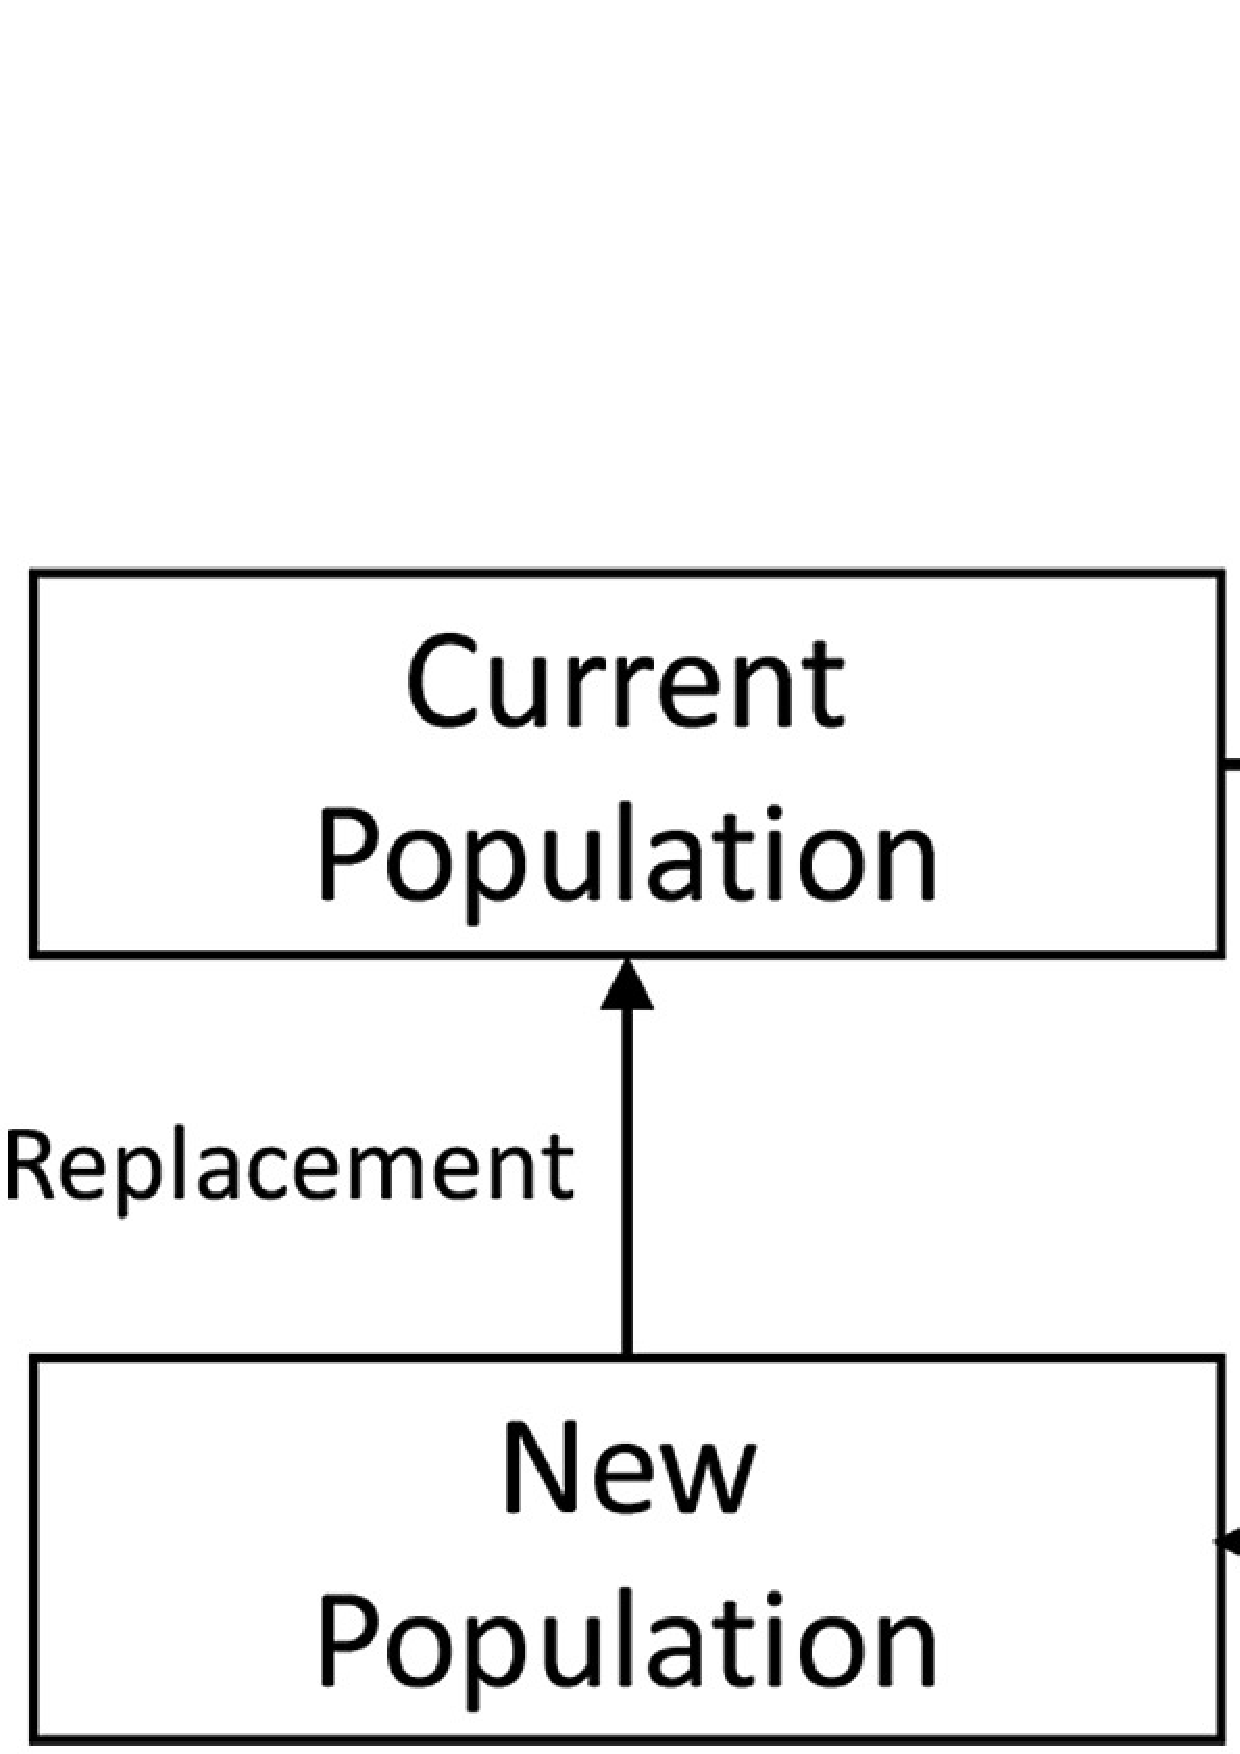
\includegraphics[scale=0.9]{gen-algo.jpg}
\end{figure} 
\end{block}
\end{frame}

\begin{frame}[c]{Framework}
\begin{figure}[ht!]
    \centering
    \includegraphics[scale=0.3]{flow.png}
\end{figure} 
\end{frame}

\begin{frame}[c]{Framework - example}

\begin{enumerate}
\item  Configuration: StyleGAN2-ffhq, GA algorithm, CLIP,  \\200 iterations
\item Input text: \textbf{a blond girl with a smile}
\item Batch after 100 iterations:
\begin{figure}[ht!]
    \centering
    \includegraphics[scale=0.15]{blondgirl.PNG}
\end{figure}
\item Final image:
\begin{figure}[ht!]
    \centering
    \includegraphics[scale=0.07]{result_blond.jpeg}
\end{figure}
\end{enumerate}
\end{frame}

\section{Experiments}

\begin{frame}{GA vs DE}
\centering
\textbf{"A yellow car in the city"}
\begin{figure}[h]
    \centering
    \subfloat[\centering genetic algorithm]{{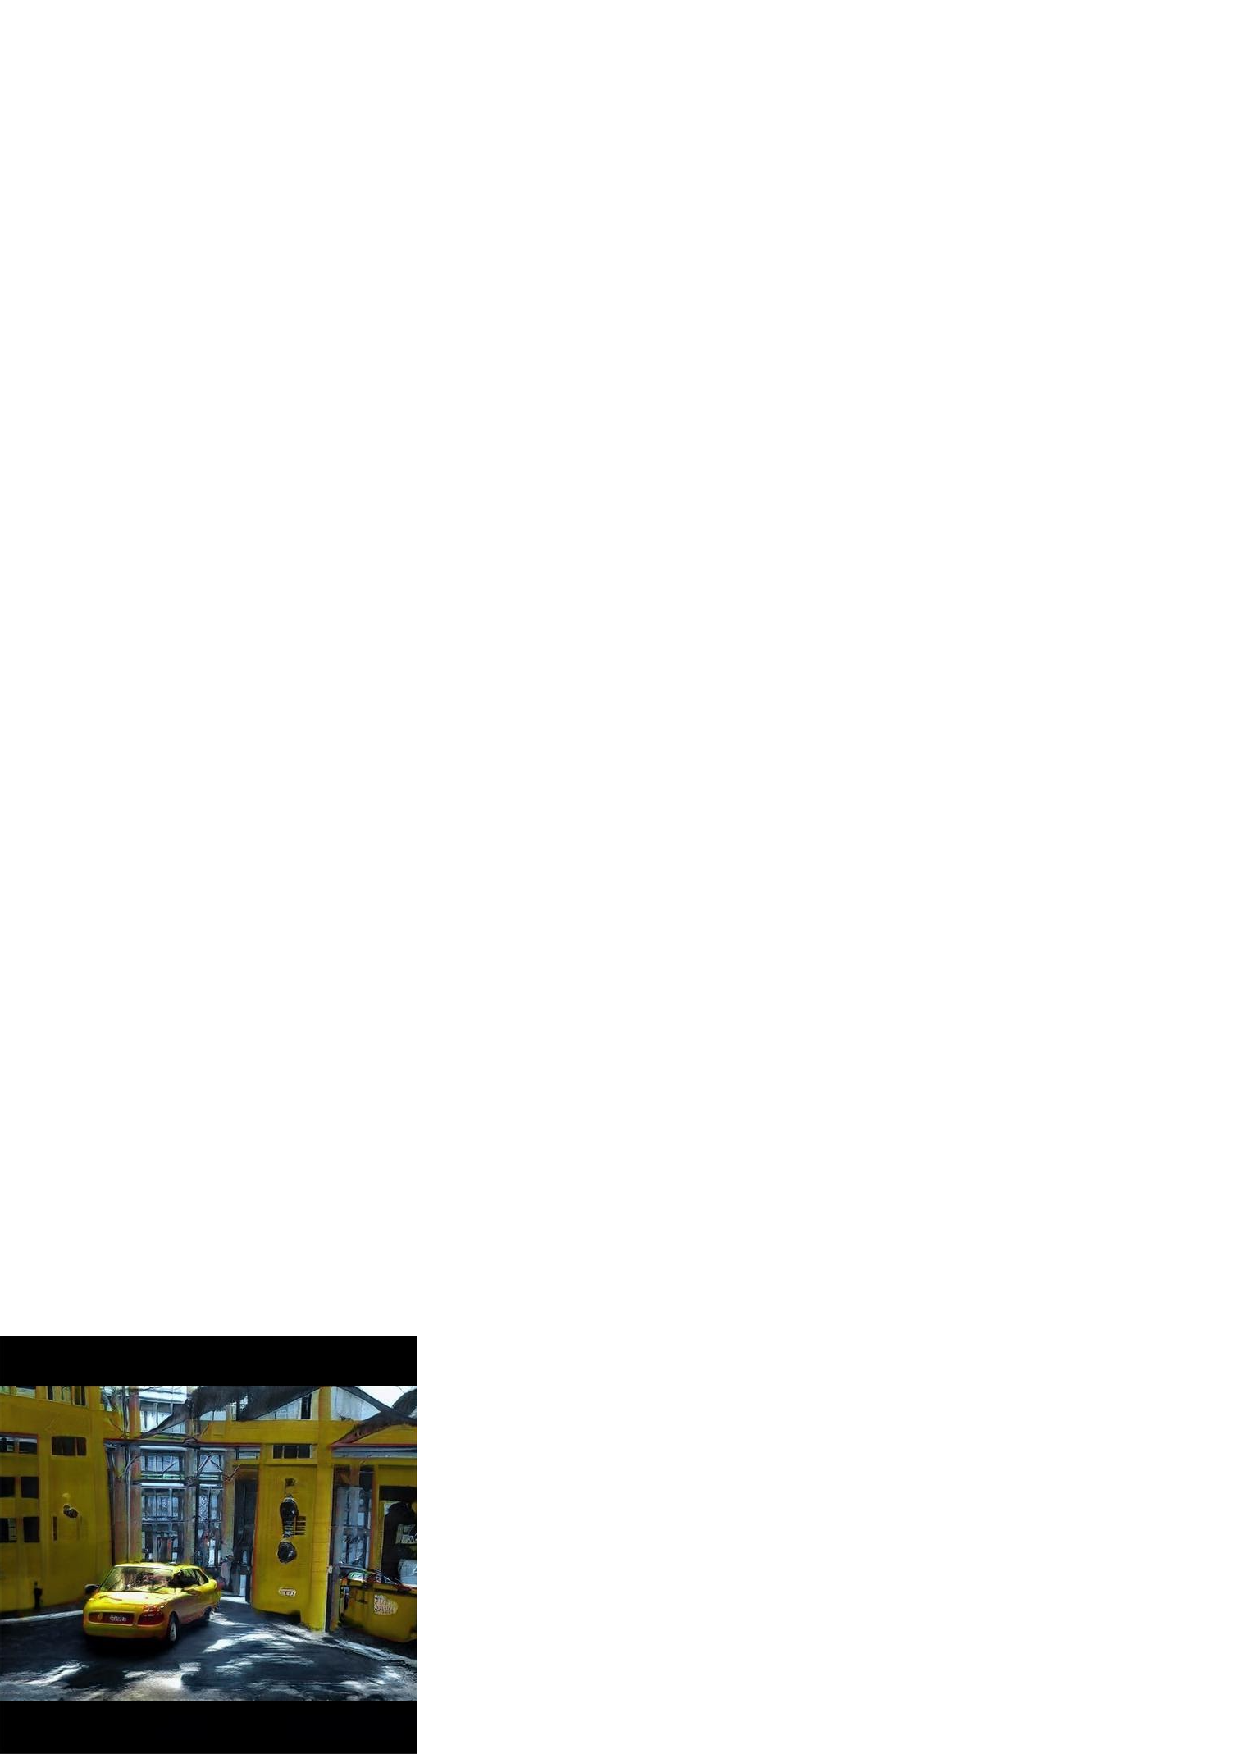
\includegraphics[width=3cm]{GA_yellowcar_final.PNG} }}
    \qquad
    \subfloat[\centering differential evolution]{{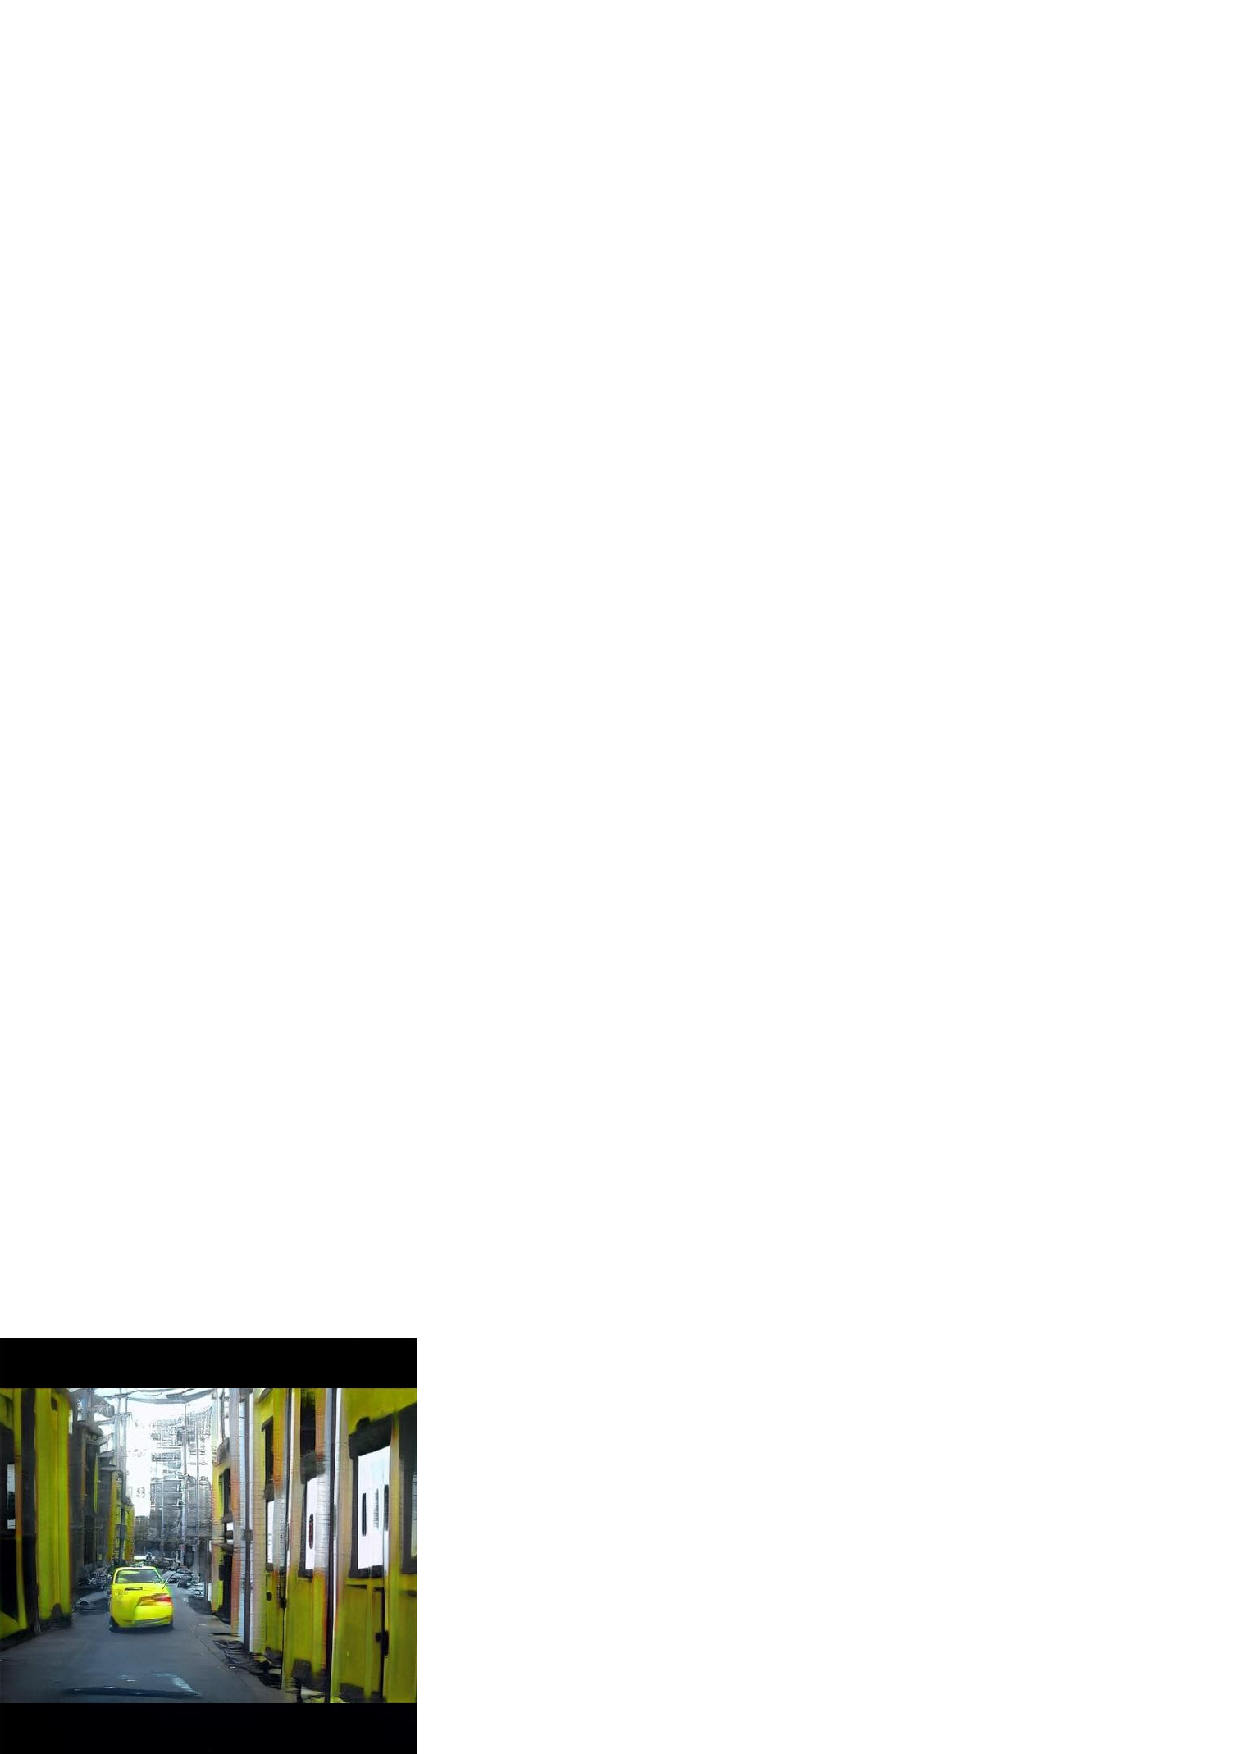
\includegraphics[width=3cm]{DE_yellowcar_final.PNG} }}
    \caption{Final images (with best score) produced by both algorithms.}
\end{figure}
\end{frame}


\begin{frame}[c]{BigGAN vs StyleGAN}
\centering
\textbf{"Red gothic church"}
\begin{figure}[H]
\centering
\begin{subfigure}[b]{0.5\textwidth}
   \includegraphics[width=1\linewidth, scale=0.15]{redgothic_stylegan.PNG}
   \caption{StyleGAN2-church}
   \label{fig:Ng1} 
\end{subfigure}
\begin{subfigure}[b]{0.5\textwidth}
   \includegraphics[width=1\linewidth, scale=0.15]{redgothic_biggan.PNG}
   \caption{BigGAN}
   \label{fig:Ng2}
\end{subfigure}
\end{figure}
\end{frame}

\begin{frame}[c]{BigGAN vs StyleGAN}
\centering
\textbf{"A clown cyclist on a moon"}
\begin{figure}[H]
\centering
\begin{subfigure}[b]{0.5\textwidth}
   \includegraphics[width=1\linewidth, scale=0.15]{clown_stylegancar.PNG}
   \caption{StyleGAN2-car}
   \label{fig:Ng1} 
\end{subfigure}
\begin{subfigure}[b]{0.5\textwidth}
   \includegraphics[width=1\linewidth, scale=0.15]{clown_biggan.PNG}
   \caption{BigGAN}
   \label{fig:Ng2}
\end{subfigure}
\end{figure}
\end{frame}

\begin{frame}[c]{Evaluation - CIFAR10}
\begin{figure}
    \centering
    \includegraphics[scale=0.3]{confusion_matrix.png}
\end{figure} 
\end{frame}

\begin{frame}[c]{Evaluation - ImageNet}
\fontsize{9}{6}\selectfont
\begin{table}[h!]
\begin{tabular}{|l|c|c|c|}
\hline
\multicolumn{1}{|c|}{\textbf{Class}} & \textbf{Positive} & \textbf{Negative} & \textbf{Accuracy (\%)}       \\ \hline
BANANA                               & 111               & 401               & {\color[HTML]{000000} 21.68} \\ \hline
CASH MACHINE                         & 124               & 388               & 24.22                        \\ \hline
HAMMER                               & 141               & 371               & 27.54                        \\ \hline
ICE CREAM                            & 3                 & 509               & {\color[HTML]{FE0000} 0.59}  \\ \hline
LLAMA                                & 36                & 476               & {\color[HTML]{333333} 7.03}  \\ \hline
MINISKIRT                            & 220               & 292               & 42.97                        \\ \hline
PIRATE                               & 5                 & 507               & 0.98                         \\ \hline
SHOPPING CART                        & 125               & 387               & 24.41                        \\ \hline
WALL CLOCK                           & 146               & 366               & 28.52                        \\ \hline
KERRY BLUE TERRIER                   & 253               & 259               & {\color[HTML]{32CB00} 49.41} \\ \hline
\textbf{TOTAL}                       & \textbf{1164}     & \textbf{3956}     & \textbf{22.73}               \\ \hline
\end{tabular}
\end{table}
\end{frame}

\begin{frame}[c]{Evaluation - ImageNet - Example}
\textbf{Llama}
\begin{figure}
    \centering
    \includegraphics[scale=0.25]{llama.png}
\end{figure} 
\end{frame}

\section{Conclusions}

\begin{frame}[c]{Conclusions}
\begin{itemize}
\item Natural continuation of this work would be to to test more algorithms and more generative models. 
\item We would also like to perform a more comprehensive analysis of phrase semantics, how the meaning of more complicated phrase is intepreted by the model and translated to latent vector.
\item Problem including new entities creation is still in the early stage of development, regarding both image and text generation, which makes it a perfect occasion to learn and develop.
\end{itemize}
\end{frame}

\end{document}
